
%(BEGIN_QUESTION)
% Copyright 2012, Tony R. Kuphaldt, released under the Creative Commons Attribution License (v 1.0)
% This means you may do almost anything with this work of mine, so long as you give me proper credit

Shade the area(s) on this graph representing the following integral (assuming each horizontal and vertical division on the graph has an incremental value of 1):

$$\includegraphics[width=15.5cm]{i01342x01.eps}$$

$$\int_{-5}^{2} (z - y) \> dx$$

Also, determine whether the numerical value of this integral is {\it positive} or {\it negative}.

\vskip 20pt \vbox{\hrule \hbox{\strut \vrule{} {\bf Suggestions for Socratic discussion} \vrule} \hrule}

\begin{itemize}
\item{} Identify some possible units of measurement for $z$, $y$, and $x$ that might fit the given integral.  Given the units you choose, which unit of measurement would go with the interval limits $-5$ and 2?
\item{} Challenge yourself by identifying {\it any other area} bounded by two of the functions on this graph and then writing an integral expression for that area.
\item{} Challenge yourself by writing an arbitrary integral expression using any one function ($y$, $w$, or $z$) or the difference between any {\it two} of those functions, and any two starting and ending points on the $x$ axis (interval limits), then shade the area on the graph represented by that expression.
\end{itemize}

\underbar{file i01342}
%(END_QUESTION)





%(BEGIN_ANSWER)

This integral has a {\it positive} value:

$$\includegraphics[width=15.5cm]{i01342x02.eps}$$

%(END_ANSWER)





%(BEGIN_NOTES)


%INDEX% Mathematics, calculus: integral (defined in a graphical sense)

%(END_NOTES)


